\documentclass[10pt,a4paper, twocolumn]{article}
%\usepackage[latin1]{inputenc}
\usepackage{listings}
\usepackage{amsmath}
\usepackage{amsfonts}
\usepackage{amssymb}
\usepackage{graphicx}
\usepackage{multirow}
\usepackage{tikz}
\usepackage[left=2.00cm, right=2.00cm, top=2.00cm, bottom=2.00cm]{geometry}
\usepackage{bm}
\usepackage[colorinlistoftodos]{todonotes}
\usepackage{xspace}
\usepackage{booktabs}
\usepackage{array}
\usepackage{dirtytalk}
\usepackage{mathtools}
\usepackage{makecell}
\usepackage{multirow}
\definecolor{on_bckgrd}{HTML}{F6BCB2}
\definecolor{off_bckgrd}{HTML}{A4D5EA}

%--- Variables ---%
\providecommand{\ve}[1]{{\bm {#1}}} %
\providecommand{\mat}[1]{{\bm {#1}}} %

%--- Operators ---%
\providecommand{\abs}[1]{\lvert{#1}\rvert}%
\providecommand{\norm}[1]{\left|\left|{#1}\right|\right|} %
\providecommand{\normal}[2]{\mathcal{N} (#1, #2)} % FDP Gauss
\providecommand{\dotp}[2]{\langle #1, #2 \rangle}
\providecommand{\mean}[1]{ \mathcal{E} \{#1\} }
\providecommand{\est}[1]{{\widehat{#1}}}
\providecommand{\cov}[1]{{\mathrm{cov}\left({#1}\right)}}
\providecommand{\corr}[1]{{\mathrm{corr}\left({#1}\right)}}
\providecommand{\vect}[1]{{\mathrm{vec}\left({#1}\right)}}
\DeclareMathOperator*{\argmin}{arg\,min}
\DeclareMathOperator*{\argmax}{arg\,max}
\DeclareMathOperator*{\diag}{\mathrm{diag}}
\DeclareMathOperator*{\Diag}{\mathrm{Diag}}
\providecommand{\geodist}[2]{{\ensuremath{d_g}}\{#1,#2\}}

%--- Other ---%
\newcommand{\Real}{\mathbb{R}}
\newcommand{\Complex}{\mathbb{C}}
\newcommand{\Natural}{\mathbb{N}}
\newcommand{\T}{\textsf{T}}
\newcommand{\x}{\times}

%--- Text modifiers ---%
\providecommand{\red}[1]{\textcolor{red}{#1}}
\providecommand{\blue}[1]{\textcolor{blue}{#1}}
\providecommand{\black}[1]{\textcolor{black}{#1}}
\providecommand{\green}[1]{\textcolor{green}{#1}}
\providecommand{\magenta}[1]{\textcolor{magenta}{#1}}

\providecommand{\mat}[1]{{\bm {#1}}}
\newcommand{\cpd}[0]{\textit{copy-draw}\xspace}
\newcommand{\cpdt}[0]{\textit{copy-draw}~test\xspace}
\newcommand{\patient}[2]{$S_{#1}^{#2}$}
\newcommand{\regtask}{RegTask\xspace}
\newcommand{\classtask}{ClassTask\xspace}
\newcommand{\speed}{v}
\newcommand{\jerk}{j}
\newcommand{\precision}{p}
\newcommand{\accel}{a}
\newcommand{\tracepos}{\vec{\ve{r}}}
\newcommand{\speeddir}{\vec{\ve{v}}}
\newcommand{\jerkdir}{\vec{\ve{j}}}
\newcommand{\precisiondir}{{{p}}}
\newcommand{\acceldir}{\vec{\ve{a}}}
\newcommand{\dir}{\phi}

%\title{Data-driven identification of acute and chronic cortical neural-markers for characterization of Parkinson's diseases symptoms}
\title{Data-driven characterization of cortical neural markers for DBS treatment of Parkinson's disease}
% non-stationarity
% acute and chronic
%
%
%
\begin{document}
\maketitle
\listoftodos

\begin{abstract}

\begin{itemize}
\item Motor performance decoding from EEG features
\item Are the identified features the same as in CSP for classifying DBS ON/OFF?
\item How are the intra-trial dynamics?
\item How are the intra-session dynamics?
\item Non trivial decoding (compare to SSD)
\item Stationarity of relevant components across sessions
\end{itemize}
\end{abstract}

\section{Introduction}

\section{Methods}
\subsection{Motor paradigm - The \cpdt}\label{sec:copydraw}
To obtain behavioral characteristics of fine motor function, we propose to use a complex hand-drawing task, termed the \cpdt. The original idea was first introduced by \cite{prichard2014effects} as a motor \mbox{skill-learning} assessment tool requiring \say{\textit{complex, synergistic, and continuous movements of multiple hand and arm muscles}}, and therefore, suitable for assessing upper-limb fine motor function affected by PD symptoms \cite{teulings1997parkinsonism, sadikov2017spirography, zham2017distinguishing}.

The experimental setup used for our study is sketched in Figure~\ref{fig:paradigm_layout}. During the \cpdt, patients sit comfortably, approximately 60\,cm in front of a 22'' screen. The dominant hand holds an electronic pen and rests on a digital drawing pad. At the beginning of a \cpd~\textit{trial}, a trace (a) composed of pseudo-letters is displayed on screen. It is composed of three predefined trace \textit{atoms} (b), which could be combined to six different traces to counter a motor habituation to any specific trace trajectory. 
To start a trial, patients were required to tap a cyan \textit{get-ready} box (c) located on the top-left corner and then proceed to the starting point of the trace, marked by a red circle (d). Reaching the start of the trace, their task was to copy-draw the trace trajectory \say{\textit{as fast and as accurately as possible}} while a diminishing visual bar indicated the time left to finish the current trial's trace. A text with this instruction (in German: \say{\textit{Bitte zeichnen Sie die Linie möglichst vollständig und exakt nach.}}) was displayed on the screen throughout the trial. No further instructions were provided, besides advising the patient not to change the precision-speed trade-off throughout the session.  Finally, we have parameterized and adapted the original \cpdt~to match the needs of our patients. For example, the time allowed to execute a trial could be adjusted such that patients were able to complete the trials on a regular basis, while keeping the task challenging.
\subsection{Characterization of tracing features}
For every \cpd~trial, two sets of kinematic and precision features could be extracted from the drawn trace: 1) directed features, embedding information about movement direction and 2) undirected features, disregarding such directional information.

\subsubsection{Directed features}  These features are based on the velocity, acceleration, and jerk of the trace and, for each trial $i$, are respectively defined as
\begin{align*}
\speeddir_k =& \frac{\tracepos_k - \tracepos_{k-1}}{\Delta t} \\
\acceldir_k =& \frac{\speeddir_k -\speeddir_{k-1}}{\Delta t}\\
\jerkdir_k =& \frac{\acceldir_k-\acceldir_{k-1}}{\Delta t}
\end{align*}
where $\lbrace \tracepos_k, \speeddir_k, \acceldir_k, \jerkdir_k \rbrace \in \Real^{2}$, with $\tracepos_k$ being the cursor coordinates on the drawing pad at time point $k$, and $\Delta t$ the time elapsed in seconds between $k-1$ and $k$.

In order to capture movement precision $\precisiondir_k$ at each time point $k$, the similarity between drawn and template traces is computed as the distance between them. To do so, each point of the drawn trace is matched to the template using dynamic time warping (DTW)\cite{berndt1994using}; subsequently, the Euclidean distance between the matched points in the drawn trace and the template is computed:
\begin{align*}
\precisiondir_k = \|\tracepos_k - \vec{\ve{t}}_m\|
\end{align*}

where $\|\cdot\| $ is the $\ell_2$-norm of the argument and $\ve{t}_m \in \Real^{2}$ is $m$-th point of the template $\ve{t}$ matched to $\tracepos_k$ using DTW.

After characterizing each point of the trace, the magnitude of each kinematic variable and the precision, i.e., $\speeddir_k, \acceldir_k, \jerkdir_k, \precisiondir_k$, for all $k$, are binned according to the spatial direction of the pen's stroke movement at time point $k$, i.e., $\dir_k =  \angle(\speeddir_k)$. The stroke movement directions were discretized into the following eight directional bins:

\begin{align*}
\mathbb{B} = \lbrace \lbrack (n-1)\pi/4; n\pi/4 ) :  n \in \Natural~|~ 1\leq n \leq 8 \rbrace,
\end{align*}
A final feature vector of each trial $i$ was obtained by averaging the elements contained in each bin of $\mathbb{B} $, as

\begin{align*}
\ve{x}^d_i \coloneqq\lbrack \langle\|\speeddir_k^{~n}\|\rangle , \langle\|\acceldir_k^{~n}\|\rangle, \langle\|\jerkdir_k^{~n}\| \rangle , \langle\precisiondir_k^{n}\rangle \rbrack^\T \in \Real^{32} 
\end{align*}

\noindent $\text{for }  n\in{\lbrace 1...8 \rbrace} \text{ and } {k:\phi_k \in \lbrack (n-1)\pi/4; n\pi/4 )}$, where $\ve{x}^d_i$ is the vector of directed features for the $i$-th trial, operator $\langle \cdot \rangle$ is the arithmetic mean, and exponent $n$ indicates the radial bin correspondence of each feature at each point $k$, as defined in $\mathbb{B}$. 

\subsubsection{Undirected kinematic features} Based on the directed features defined above, a set of undirected features is also considered. In this case, the average magnitude for each of the variables  $\speeddir_k, \acceldir_k, \jerkdir_k, \precisiondir_k$ is computed for the entire trial duration, thus, disregarding any movement direction information.  Specifically, for the $i$-th trial, the four dimensional undirected feature vector $\ve{x}^u_i$ is defined as:

\begin{align*}
\ve{x}^u_i \coloneqq \lbrack \langle\|\speeddir_k\|\rangle , \langle\|\acceldir_k\|\rangle, \langle\|\jerkdir_k\| \rangle , \langle\precisiondir_k\rangle  \rbrack^\T \in \Real^{4}\text{, for all}~~k
\end{align*}




\subsection{Supervised dimensionality reduction for scoring PD-relevant motor function}\label{sec:lda}
Using an universal single feature of motor execution, as derived from the \cpdt, is not sufficient for characterizing fast DBS-induced changes in motor function for all patients, due to the heterogeneity of the disease symptoms. For example, for a patient affected by bradykinesia or rigor, speed will likely be a relevant proxy of motor function, whereas jerk will be so for a patient mostly affected by tremor. On the other hand, all motor execution features could be used simultaneously; however, such \textit{high}-dimensional representation of fine motor function also implies an interpretability problem, because it becomes difficult to determine the optimal weighting of the features in order to obtain a global reliable and sensitive motor-score that encompasses DBS-induced changes in motor control, for each patient individually.

To tackle these challenges, dimensionality reduction algorithms can be used in order to find representative subspaces that capture the essential characteristics of the underlying motor dynamics. One classic supervised dimensionality reduction algorithm is the linear-discriminant analysis (LDA) \cite{duda2012pattern}. LDA seeks to find a projection from the high-dimensional feature space to a one-dimensional subspace, which optimizes the separation of data points by the given class labels. While such class labels are generally not available in hand motor assessment, they are in the specific case of executing the \cpdt~under trial-wise varying DBS conditions. Here we can assume that the highest variability in motor function is induced by the DBS condition, i.e., DBS-on or DBS-off. Training an LDA model using the DBS condition (on/off) as class labels, a low-dimensional subspace of the high-dimensional behavioral features can be found, which delivers an interpretable representation of the DBS-induced effects on motor function.

Let $\mat{X} = [\ve{x}^\T_1 \ldots \ve{x}^\T_N] \in \Real^{N\times M}$ be a matrix containing N normally distributed M-dimensional feature vectors $\ve{x}_i \in \{\ve{x}^d_i, \ve{x}^u_i\} \sim  \mathcal{N}(0,\mat{I})$, with $\mat{I} \in \Real ^{M\times M}$ being the identity matrix; and  $\ve{w} \in \Real^d$ a vector which projects the features onto a scalar variable. Then, the LDA objective function to find a subspace with the maximum separability between classes and minimum variance within classes is formulated as
\begin{align*}
\argmax_\ve{w} \left\lbrace \frac{\ve{w}(\ve{\mu}_{on}-\ve{\mu}_{off})(\ve{\mu}_{on}-\ve{\mu}_{off})^\T\ve{w}^\T}{\ve{w}(\mat{\Sigma}_{on}+\mat{\Sigma}_{off})^\T\ve{w}^\T} \right\rbrace,
\end{align*}

where $ \{\ve{\mu}_{on},\ve{\mu}_{off}\} \in \Real^{d}$ are the mean vectors and  $ \{\mat{\Sigma}_{on},\mat{\Sigma}_{off}\} \in \Real^{d\times d}$ the covariance matrices of the features computed from trials executed during DBS conditions on and off, respectively.

Assuming homoscedasticity for the underlying background brain processes of the on and off classes, which cause feature variation beyond class-defined averages, the formulation can be simplified with $\mat{\Sigma}_{on} = \mat{\Sigma}_{off} = \mat{\Sigma}$. Subsequently, solving the optimization problem is equivalent to solving the following generalized eigenvalue problem:
\begin{align}\label{eq:eig_lda}
(\ve{\mu}_{on}-\ve{\mu}_{off})(\ve{\mu}_{on}-\ve{\mu}_{off})^\T \ve{w} = \lambda\mat{\Sigma}\ve{w}
\end{align}

After finding an optimal projection vector $\ve{w}$ by solving \eqref{eq:eig_lda}, a scalar motor-score $y_i$ is obtained for every trial $i$ by projecting the corresponding feature vector $\ve{x}_i \in \{\ve{x}^d_i, \ve{x}^u_i\}$, onto the space spanned by $\ve{w}$:

\begin{align}\label{eq:score_projection}
y_i = \ve{w}^\T\ve{x}_i
\end{align}

If the goal is to classify the $i$-th trial, the corresponding class for the $i$-th trial can be estimated according to the class mean projection onto $\ve{w}$:

\begin{align*}
\text{class of $i$-th trial}=\begin{cases}
\text{on}, & \text{if $y_i \geq \ve{w}(\ve{\mu}_{on}+\ve{\mu}_{off})/2$}\\
\text{off}, & \text{otherwise.}
\end{cases}
%
\end{align*}
Furthermore, additional information about the relevance of each feature in the projected subspace can be extracted by computing 
\begin{align}\label{eq:patterns}
\ve{a} = \mat{\Sigma}\ve{w}
\end{align}

where $\ve{a} \in \Real ^ {d}$ contains the activation patterns of the optimized vector $\ve{w}$, describing the contribution of the original features in constructing the space spanned by vector $\ve{w}$ \cite{haufe2014interpretation}.

When the feature dimensionality is not substantially smaller than the number of training samples, the estimated empirical covariance matrix (sample covariance matrix) $\mat{\Sigma}_s$ tends to be distorted. One way of addressing this problem is to regularize the final estimated covariance matrix towards the unit hypersphere by

\begin{align*}
\mat{\Sigma} = (1-\lambda)\mat{\Sigma}_s + \lambda\mat{I}
\end{align*}

where $\lambda$ is the regularization parameter; which can be estimated analytically using the approach proposed by Ledoit and Wolf \cite{ledoit2004well}.
\subsection{Decoding of PD-relevant motor performance}

Based on the assumption that relevant NM can be found in cortical and subcortical signals, it can be hypothesized that underlying EEG sources may contain relevant information about NMs for PD.  Following, we will describe how these informative oscillatory sources can be recovered from overlapping confounds and noisy EEG signals in a short-timescale, single-trial basis. 

\subsubsection{Forward model of EEG generation}
\label{par:modeling}
%\begin{figure*}[h!]
Due to volume conduction, non-invasive imaging techniques, as EEG, measure electrical brain activity generated by superimposed hidden brain sources. In general, the properties of such superposition is linear, thus, it can be described as a linear combination of neural generators, which can be modeled as follows.

Let $\mat{X}\negmedspace\in\negmedspace \Real^{N_c \times N_t}$ be a multivariate variable to describe data of brain activity measured in the EEG sensor space, where $N_t$ is the number of time samples and $N_c$ the number of sensors. Furthermore, let $\mat{S} \negmedspace\in\negmedspace \Real^{N_s \times N_t}$ describe the time course of $N_s$ neural sources, where $N_s$ describes the number of hidden neural sources considered. Then, the general EEG generative model can be written as: 
\begin{align}\label{eq:genModel}
\mat{X}=\mat{A}\,\mat{S} + \mat{E} \;.
\end{align} 
In this model, matrix $\mat{A}\negmedspace\in\negmedspace \Real^{N_c \times N_s}$ describes the projection of the sources to the sensor space, where the columns of $\mat{A}$, $\ve{a} \negmedspace\in\negmedspace \Real^{N_c}$, are referred to as \emph{spatial patterns}. Furthermore, the matrix $\mat{E}$ contains spatially and temporally uncorrelated noise to model measurement noise. 

An estimation of the time-course of a source component, i.e.\ $\hat{\ve{s}}$, can be extracted from the measurements by way of a \emph{spatial filter} $\ve{w} \in \Real^{N_c}$, which projects the data from sensor space into source space. Thus we have $\hat{\ve{s}} = \ve{w}^\top\mat{X}$.
%A source component $\hat{\ve{s}}_X=\ve{w}^\top\mat{X}$
%can be extracted from the time course of the sensor data by applying a  spatial filter $\mat{w}\negmedspace\in\negmedspace\Real^{N_c \times 1}$, which projects data from the sensor space to the source space. 
For many problems, such a spatial filter $\mat{w}$ is not known a priori and must be estimated from the data. However, once a spatial filter (or an entire set thereof, denoted by $\mat{W} \in \Real^{N_c \times N_s}$, where each column $\ve{w}$ represents a single spatial filter) has been obtained, an estimate of the corresponding spatial patterns can be computed via the relation $ \hat{\mat{A}} = \mat{C} \mat{W} \left( \mat{W}^\top \mat{C} \mat{W} \right)^{-1} $, where $\mat{C} \in  \Real^{N_c \times N_c} $ denotes the spatial covariance matrix of the data $\mat{X}$. See \cite{haufe2014interpretation} for further details on the relation between spatial filters and spatial patterns.  

\subsubsection{Common spatial patterns (CSP)}

The CSP algorithm is an established supervised method in the BCI community, used in classification tasks for constructing a set of $N_c$ spatial filters $\mat{W}_{CSP} \in \Real^{N_c \times N_c}$ that optimally discriminates epochs of two classes characterized by differing band-power features, where the labels are defined as $\ve{y} \in \lbrace 1,2 \rbrace$, corresponding to a discretization of the continuous label $\ve{z}$.

Assuming that M/EEG data $\mat{X}$ have been bandpass filtered to the frequency band of interest and segmented into a set of $N$ epochs, where $\mat{X}(e)$ represent the $e$-th epoch of the M/EEG data, the CSP objective function is mathematically formalized as
\begin{align}
\underset{\ve{W}_{CSP}}{\operatorname{argmax}} \, \, \, \frac{ \ve{W}_{CSP}^\T \left( \ve{C}_1 -  \ve{C}_2\right)\ve{W}_{CSP}}{\ve{W}_{CSP}^\T\, \ve{C} \, \ve{W}_{CSP}}.
\end{align}
with the spatial covariance matrices of classes one and two defined as $\mat{C}_{1,2} = N^{-1}_{1,2}\sum_e^N\mat{X}_{1,2}(e)\mat{X}_{1,2}(e)^\T$ and with $\ve{C}$ being the pooled spatial covariance matrix. It can be shown that a solution to the CSP optimization problem can be found by solving the  generalized eigenvalue problem 

\begin{align}\label{eq:eig_csp}
\mat{W}_{CSP}^\T\left(\mat{C}_1 - \mat{C}_2\right) = \mat{\Lambda} \mat{W}_{CSP}^\T\mat{C}
\end{align}

with $\ve{W}_{CSP}$ being a matrix containing (column-wise) the eigenvectors (i.e., spatial filters) which are related to the eigenvalues provided by the entries of the main diagonal of $\mat{\Lambda} \in \Real^{N_f \times N_f}$.

For our tests, we reduced the full filter matrix to $\est{\mat{W}}_{CSP}\in \Real^{Nc \times 2}$. Thus, it contains two eigenvectors only, one corresponding to the largest and one to the smallest eigenvalues in $\mat{\Lambda}$, representing each class respectively. The selection of the number of CSP filters is an important hyperparameter for obtaining an optimal decoding performance. However, according to \cite{blankertz2011single}, a good rule of thumb indicates that between 2 and 8 filters are likely to deliver a good performance.

Note that a spatial filters derived by CSP does not deliver an estimate of the target variable $\est{z}(e)$ yet. To derive estimates of the target variable, we thus trained a regularized LDA (rLDA) classifier on the power features (delivered by $\Theta_x(e) = \operatorname{var}[\hat{\ve{s}}](e)$) of the spatially filtered data $\hat{\ve{s}}(e)=\est{\mat{W}}_{CSP}^\top\mat{X}(e)$\cite{blankertz2011single}.

\subsubsection{Source Power Co-modulation --- SPoC}
\label{par:spoc}
The source power co-modulation (SPoC) method introduced in~\cite{dahne2014spoc} utilizes a supervised regression approach in order to estimate a set of spatial filters $\mat{W}$. The method assumes that the recorded data $\mat{X}$ has been pre-filtered to a narrow frequency band, which contains the oscillatory source of interest. 

Based on data of multiple epochs $e$, a filter $\mat{w}$ is optimized such that the power of an epoch $\Theta_x(e) = \operatorname{var}[\hat{\ve{s}}](e)$ of the spatially filtered data $\hat{\ve{s}}=\mat{w}^\top\mat{X}$, maximally covaries with a known, epoch-wise defined univariate target variable $z(e)$. For the sake of simplicity in the notation, $\hat{\ve{s}}$ will be noted as $\ve{s}$, hereafter.
 
%\end{align}
It can be shown that solving the optimization problem described above, is equivalent to solving the following generalized eigenvalue problem
\begin{align}\label{eq:eig_spoc}
\mat{C}_z\mat{W} = \mat{\Lambda}\mat{C}\mat{W}
\end{align}
where $\mat{C}_z = \left<\mat{C}(e)z(e)\right>$, $\mat{C} = \left<\mat{C}(e)\right>$, and $\left<\mat{C}(e)\right>$ and $\left<\mat{C}(e)z(e)\right>$ are, respectively, the weighted covariance and covariance of $\mat{X}$, averaged across epochs $e$: $\mat{C}(e) = \mat{X}(e)\mat{X}(e)^\T$; and $\mat{\Lambda} \in \Real^{N_c\times N_c}$ is a matrix containing the corresponding eigenvalues in the main diagonal.

Given a spatial filter $\mat{w}_{tr}$ determined on training data $tr$, the true target variable $z$ can subsequently be approximated on a single-trial basis for unseen test data ($te$) epochs $\mat{X}_{te}$ via $\hat{z}(e) = \operatorname{var}[\mat{w}_{tr}^\top\mat{X}_{te}(e)]$. 


\section{Experimental setup}
\subsection{Patients}
The study was approved by the local ethics committee at the University Medical Center Freiburg and was conducted according to the Declaration of Helsinki. All patients received detailed information about the study and provided written informed consent prior to participation.

\subsection{Study design}
Seven PD patients (\patient{1,~\ldots,~7}{}) were bilaterally implanted in the STN with directional DBS electrodes (Vercise Cartesia \texttrademark Boston Scientific, Marlborough, MA, USA). Implantation trajectory and target location were planned using pre-operative CT and sMRI information, and intraoperative microelectrode recordings. The dorsolateral motor area of the STN was targeted and the leads were placed such that the dead space between the segmented electrodes of the implanted lead were located at the optimal intraoperative stimulation site. Typically this resulted in a further contact (ring) above the STN in the field of Forel. The lead locations were intraoperatively checked with lateral x-rays and post-operatively using helical CT and fusion back to the planning data (MRI).

After implantation, DBS leads were kept externalized during four days following surgery. On day four, leads were internalized and the pulse generator was implanted. In addition to a short \cpdt{} familiarization session, each patient participated in five EEG experimental sessions: one \textit{pre-session} executed a day before lead implantation, three \textit{sub-acute} sessions (\patient{}{+1,+2,+3}) on the three days following lead implantation---with concurrent recording of STN-LFP signals---, and one \textit{sub-chronic} session (\patient{}{c}) approximately 4 weeks after implantation surgery, during the first inpatient control visit. Throughout the text, we use the notation \patient{a}{b} to note the b-th session executed for patient a. So for example, \patient{5}{+3} indicates the session executed with patient 5, 3 days after lead implantation.

Since the scope of our contribution is the analysis of experimental sessions where the \cpdt{} was performed under varying DBS-on and -off, a detailed description in which \cpdt{} was not executed or executed under constant DBS conditions is omitted. A description of the 16 session that we will deal with here, can be found in Table \ref{tab:all_cpd_sessions_descrip}
\begin{table*}
\resizebox{\textwidth}{!}{
\begin{tabular}{cccccccccccc}
%\cellcolor{gray!25}

%%%%%%%%%%%%%%%%%%%%%%%%%%%%%%%%%%%%%%%%%%%%%%%
%%%%%%%%%%-------- PATIENT 1 ---------%%%%%%%%%
%%%%%%%%%%%%%%%%%%%%%%%%%%%%%%%%%%%%%%%%%%%%%%%
\textbf{Subject} &	\textbf{Session} & \textbf{Age} & \textbf{Sex} &  \textbf{Medication} & \textbf{DBS parameters}& \makecell{\textbf{Trial} \\ \textbf{duration}} & \textbf{N trials} &  \makecell{\textbf{Preimplantation} \\ \textbf{UPDRS-III}} & \textbf{T} & \textbf{B} & \textbf{R}\\
\midrule[2pt]
 \addlinespace
\multirow{2}{*}{\patient{1}{}} & +2 &\multirow{2}{*}{55} &\multirow{2}{*}{M} & \makecell{normal acting l-Dopa at +26\,min \\ 
 	and fast acting l-Dopa at +43\,min} & 3\,mA, uni & \multirow{2}{*}{7.5\,s} &144 &\multirow{2}{*}{25 (med-on)} & 0 & +2 & +2\\ 
 
 \addlinespace
& c &  & & 
 \makecell{fast acting l-Dopa at +15\,min} & 2.4\,mA, bi&&216& & \multicolumn{3}{c}{n/a}\\ 
\midrule[0.5pt]
 \addlinespace
 
 
 %%%%%%%%%%%%%%%%%%%%%%%%%%%%%%%%%%%%%%%%%%%%%%%
 %%%%%%%%%%-------- PATIENT 2 ---------%%%%%%%%%
 %%%%%%%%%%%%%%%%%%%%%%%%%%%%%%%%%%%%%%%%%%%%%%%
 
\multirow{2}{*}{\patient{2}{}} & +2 & \multirow{2}{*}{54} &\multirow{2}{*}{F} & \multirow{2}{*}{medication off} &  \multirow{2}{*}{6\,mA, uni} & \multirow{2}{*}{6\,s} & 144 & \multirow{2}{*}{18} & +2 & +2 & +2\\
 \addlinespace
& c & &  & && &168 & & +3 & 0 & +2  \\
 %\addlinespace
 \midrule[0.5pt]
 \addlinespace
 
%%%%%%%%%%%%%%%%%%%%%%%%%%%%%%%%%%%%%%%%%%%%%%%
%%%%%%%%%%-------- PATIENT 3 ---------%%%%%%%%%
%%%%%%%%%%%%%%%%%%%%%%%%%%%%%%%%%%%%%%%%%%%%%%%
\patient{3}{} & c & \multirow{1}{*}{56} &\multirow{1}{*}{M} & medication off & 6\,mA,  uni & 7.5\,s &120 & 41 & \multicolumn{3}{c}{n/a}\\

\midrule[0.5pt]
 \addlinespace

%%%%%%%%%%%%%%%%%%%%%%%%%%%%%%%%%%%%%%%%%%%%%%%
%%%%%%%%%%-------- PATIENT 4 ---------%%%%%%%%%
%%%%%%%%%%%%%%%%%%%%%%%%%%%%%%%%%%%%%%%%%%%%%%%
\multirow{4}{*}{\patient{4}{}} & +2 & & & retarded l-Dopa at -150\,min & 6.5\,mA, uni & \multirow{4}{*}{6\,s}&168& \multirow{4}{*}{23} &  0 & 0 & +1 \\ 
 \addlinespace
 
 & +3 & 44 & M & retarded l-Dopa at -330\,min & 5\,mA, uni &&168 && 0 & 0 & +1 \\
 \addlinespace
 
& c & & & \makecell{normal acting l-Dopa combined with\\ COMT-Inhibitor (Entacapone) at -210\,min} & 3.5\,mA, uni, 30\,$\mu$s& &156 && 0 & +1 & +2 \\
\midrule[0.5pt]
\addlinespace

%%%%%%%%%%%%%%%%%%%%%%%%%%%%%%%%%%%%%%%%%%%%%%%
%%%%%%%%%%-------- PATIENT 5 ---------%%%%%%%%%
%%%%%%%%%%%%%%%%%%%%%%%%%%%%%%%%%%%%%%%%%%%%%%%
\multirow{4}{*}{\patient{5}{}} & +2 & & & retarded l-Dopa at -300\,min & 6.5\,mA, uni & \multirow{4}{*}{6\,s}& 144 & \multirow{4}{*}{33} &  0 & +1 & +1 \\ 
\addlinespace

& +3 & 69 & M & retarded l-Dopa at -210\,min & 6.5\,mA, uni &&144 && +1 & +1 & +2 \\
\addlinespace

& c & & & \makecell{normal acting l-Dopa -660\,min} & 6.0\,mA, uni& &192 && 0 & +1 & +1 \\
\midrule[0.5pt]
\addlinespace

%%%%%%%%%%%%%%%%%%%%%%%%%%%%%%%%%%%%%%%%%%%%%%%
%%%%%%%%%%-------- PATIENT 6 ---------%%%%%%%%%
%%%%%%%%%%%%%%%%%%%%%%%%%%%%%%%%%%%%%%%%%%%%%%%
\multirow{2}{*}{\patient{6}{}} & +2 & \multirow{2}{*}{63} & & retarded l-Dopa at -330\,min & 3\,mA, uni & \multirow{2}{*}{9\,s}&144& \multirow{2}{*}{35} &  +1 & +2 & 0 \\ 
\addlinespace

& c & & & medication off & 3.5\,mA, uni& &192 && 0 & +2 & +1 \\
\midrule[0.5pt]
\addlinespace
%%%%%%%%%%%%%%%%%%%%%%%%%%%%%%%%%%%%%%%%%%%%%%%
%%%%%%%%%%-------- PATIENT 7 ---------%%%%%%%%%
%%%%%%%%%%%%%%%%%%%%%%%%%%%%%%%%%%%%%%%%%%%%%%%
\multirow{4}{*}{\patient{7}{}} & +2 & & & n/a & 4.5\,mA, uni & 9\,s&168& \multirow{4}{*}{34} &  0 & 0 & +2 \\ 
\addlinespace

& +3 & 55 & M & retarded l-Dopa at -330\,min & 5\,mA, uni & 6\,s&168 && \multicolumn{3}{c}{n/a} \\
\addlinespace

& c & & & \makecell{normal acting l-Dopa -660\,min} & 3.5\,mA, uni& 7.5\,s &192 && 0 & +2 & +2 \\

\bottomrule[0.5pt]
\vspace{0.2cm}
\end{tabular}}
\caption{Description of the \cpd~sessions analyzed. Unless otherwise indicated, DBS was performed with a pulse width of 60\,$\mu$s and frequency of 130\,Hz. The STN ipsilateral to the dominant hand was stimulated, when DBS was performed, unless bilateral stimulation was applied, which is indicated. Medication intake times are relative to the experiment start. UPDRS-III scores where obtained---unless otherwise indicated---in medication off, several days prior to the implantation surgery. Tremor (T), Bradykinesia (B), and Rigor (R) scores are given relative to the DBS-off baseline, ranging from 0 (no improvement), to +3 (complete symptom suppression). n/a marks unavailable information.}
\label{tab:all_cpd_sessions_descrip}
\end{table*}

\subsection{The \cpd~ session design}\label{sec:cpd_session_design}
A \cpd~session is constituted by a series of \textit{blocks}, with each block comprising 12 \cpd~\textit{trials} (see Section~\ref{sec:copydraw}). Within a block, DBS is either on or off, but this DBS condition is alternated between blocks. For each session, at least 10 \cpd~blocks were executed. Additional blocks were performed depending on the fatigue level reported by each patient. The patient-specific trial duration are reported in Table~\ref{tab:exp_sessions_interleaved}. Furthermore, between trials, a brief self-timed pause was allowed. Similarly, after each block, a longer pause was provided.

\subsection{DBS parameters and dopaminergic medication}
DBS amplitude was adjusted for each patient individually to a level of 0.5\,mA below side-effects onset but maximally at a level of 6.5\,mA. The electric field generated possessed an omnidirectional bipolar pattern, with the top unsegmented and adjacent segmented electrodes used as anode and cathode, respectively. Even though, chronic DBS therapy is typically performed using a unipolar pattern, we decided to apply a bipolar pattern in order to reduce the artifacts elicited in the concurrent LFP and EEG signals recorded during the experiments. During the sessions in the acute phase, DBS was performed unilaterally due to hardware limitations. During the subchronic phase, bilateral stimulation was possible but we opted for unilateral DBS for the sake of consistency with the sessions during the acute phase.

During the acute phase, DBS was always off, except during our experimental sessions, where it was turned on according to the stimulation protocol described in Section \ref{sec:cpd_session_design}. During the subchronic phase, DBS was generally on, and was turned off only 30 to 60 minutes prior to the beginning of our experimental sessions and was turned on/off according to the same stimulation protocol as in the experimental sessions during the acute phase.

Dopaminergic medication was scheduled in such a way that its effects on motor function were minimized. An absolute medication-off state was avoided depending on the patient, due to a prohibitively high level of discomfort caused by the lengthy sessions. The medication plan was managed patient- and session-wise. Its details can be found in Table~\ref{tab:all_cpd_sessions_descrip}.

%\begin{figure}[h!]
%\centering
%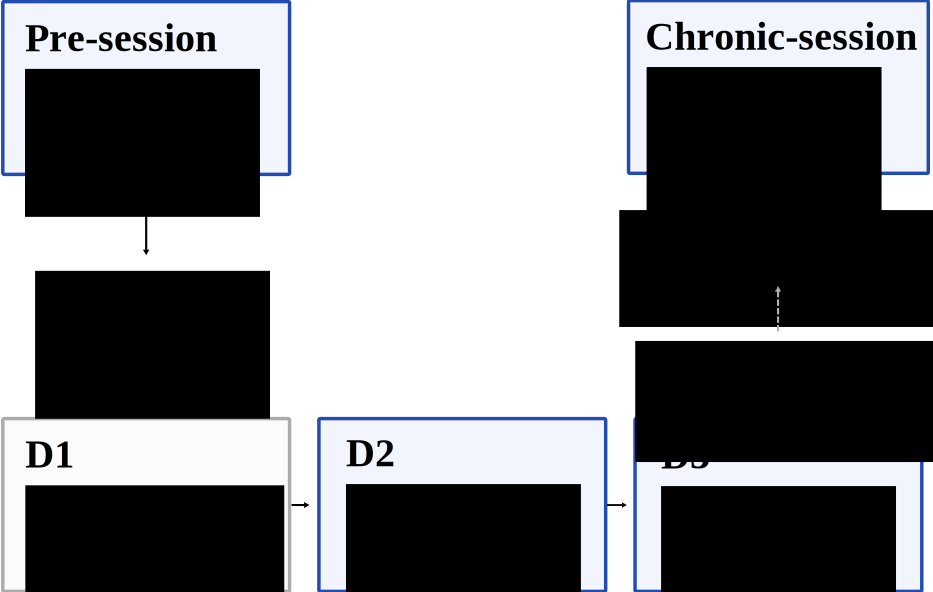
\includegraphics[width=0.45\textwidth]{figures/all_sessions}
%\caption{Overview of all experimental sessions carried out by the patients.}
%\label{fig:sessions_overview}
%\end{figure}

\subsection{Acquisition of electrophysiological signals}

EEG signals were recorded from passive Ag/AgCl electrodes (EasyCap GmbH, Germany) placed according to the extended 10-10 system. Impedances were kept below 20\,k$\Omega$. All channels were referenced against the nose during recording. The EEG signals were registered by BrainAmp DC amplifiers (Brain Products GmbH, Germany) at a sampling rate of 1\,kHz, with an analog lowpass filter of 250\,Hz applied before digitization.

For \patient{}{+2,+3}, patient-specific fronto-central-parietal areas of the scalp were unavailable for EEG placement due to the surgical wound, consequently, EEG signals were recorded from a number of electrodes that varied from patient to patient. An example of a resulting EEG configuration can be seen in Figure \ref{fig:paradigm_layout}.

Additional to EEG signals, electromyographic activity of the dominant hand, fingertip pulse wave, and bilateral STN-LFP signals ere also recorded. However, their will be dealt with in future contributions, so we will omitted here extensive description thereof.

\begin{figure*}[h!]
\centering
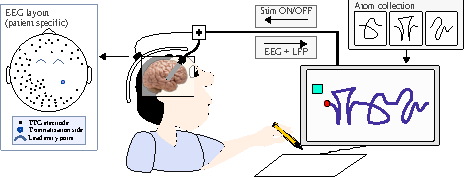
\includegraphics[width=0.8\textwidth]{figures/paradigm_layout}
\vspace{-12pt}
%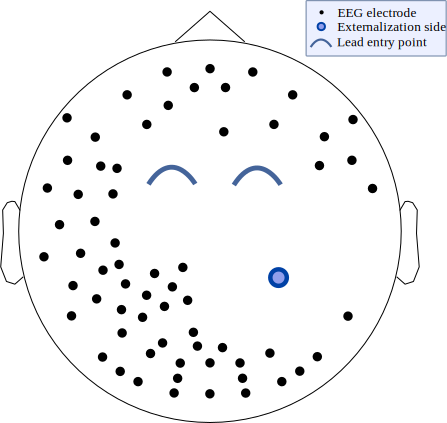
\includegraphics[width=0.4\textwidth]{figures/electrode_layout}
%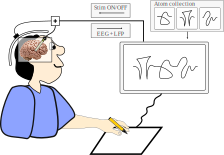
\includegraphics[width=0.5\textwidth]{figures/paradigm}
\caption{Right: Illustrative EEG layout used for one of the patients. Electrodes were placed over the entire scalp, avoiding incision sites used for DBS electrode implantation and externalization.}
\label{fig:paradigm_layout}
\end{figure*}


\section{Results}
\subsection{Modulation of motor-performance}
Figure \ref{fig:behavioral_all} shows the $PL$ score achieved by the patients in all the sessions. Complex medication-stimulation interaction can be seen for many of the recordings. For example, in session P1-D2, DBS does not have an evident effect in motor performance at the beginning of the session, but after intake of dopaminergic medication, a clear difference between DBS ON and OFF may be observed


%\begin{figure*
%	\centering
%	\def \subplotwidth {0.24\textwidth}
%	
\begin{figure}
	\centering
	\def \subplotwidth {0.24\textwidth}
\begin{tabular}{cc|c}

\includegraphics[width=\subplotwidth]{./figures/histogram_labels/histogram_labels_VPpcac_d2}& & \includegraphics[width=\subplotwidth]{./figures/histogram_labels/histogram_labels_VPpcac_d4}\\
\includegraphics[width=\subplotwidth]{./figures/histogram_labels/histogram_labels_VPpcad_d2}& & \includegraphics[width=\subplotwidth]{./figures/histogram_labels/histogram_labels_VPpcad_d4}\\
& & \includegraphics[width=\subplotwidth]{./figures/histogram_labels/histogram_labels_VPpcae_d4}\\
\includegraphics[width=\subplotwidth]{./figures/histogram_labels/histogram_labels_VPpcaf_d2}& \includegraphics[width=\subplotwidth]{./figures/histogram_labels/histogram_labels_VPpcaf_d3}& \includegraphics[width=\subplotwidth]{./figures/histogram_labels/histogram_labels_VPpcaf_d4}\\
\includegraphics[width=\subplotwidth]{./figures/histogram_labels/histogram_labels_VPpcag_d2}& \includegraphics[width=\subplotwidth]{./figures/histogram_labels/histogram_labels_VPpcag_d3}& \includegraphics[width=\subplotwidth]{./figures/histogram_labels/histogram_labels_VPpcag_d4}\\
\includegraphics[width=\subplotwidth]{./figures/histogram_labels/histogram_labels_VPpcah_d2}& & \includegraphics[width=\subplotwidth]{./figures/histogram_labels/histogram_labels_VPpcah_d4}\\
\includegraphics[width=\subplotwidth]{./figures/histogram_labels/histogram_labels_VPpcaj_d2}& \includegraphics[width=\subplotwidth]{./figures/histogram_labels/histogram_labels_VPpcaj_d3}& \includegraphics[width=\subplotwidth]{./figures/histogram_labels/histogram_labels_VPpcaj_d4}\\
\end{tabular}
\caption{Motor performance}
\end{figure}
%	\caption{motor performance}
%\end{figure*}

\begin{table}
	\centering
	\small
	\begin{tabular}{c|ccc}
DAI	& +2 & +3 & c \\
\midrule[2pt]
\patient{1}{} &	0.76 & n/a & 0.80 \\
\patient{2}{} &	0.95 & n/a & 0.64 \\
\patient{3}{} &	n/a & n/a & 0.76 \\
\patient{4}{} &	0.61 & 0.56 & 0.64 \\
\patient{5}{} &	0.67 & 0.60 & 0.80 \\
\patient{6}{} &	0.75 & n/a & 0.80 \\
\patient{7}{} &	0.64 & 0.67 & 0.65 \\
\end{tabular}
	\caption{motor performance}
\end{table}

%\subsection{Identification of artifactual SPoC and CSP components}

%\begin{figure}
%\caption{Examples of artifacts (spectrum, spatial patterns and time series)}
%\end{figure}


\subsection{Predictive cortical oscillatory components}
\begin{figure*}
	\centering
\def \subplotwidth {0.24\textwidth}
\begin{tabular}{cc|c}
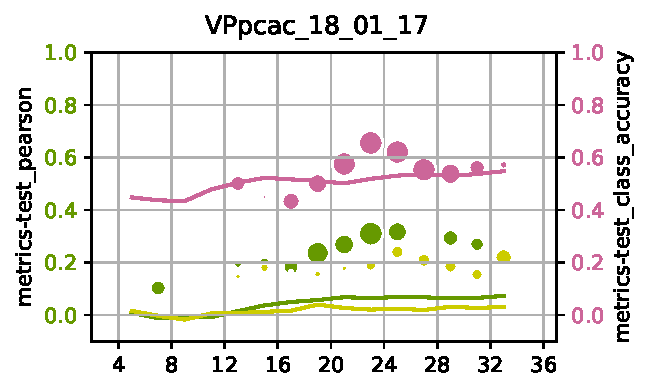
\includegraphics[width=\subplotwidth]{./figures/csp_spoc_incommon/bubble_csp_spoc_incommon_VPpcac_d2_nolegend}& & 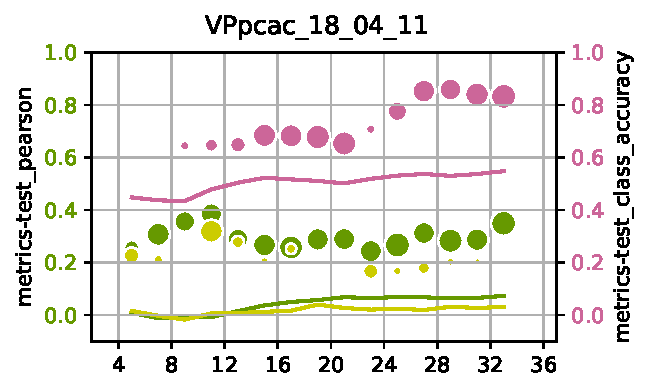
\includegraphics[width=\subplotwidth]{./figures/csp_spoc_incommon/bubble_csp_spoc_incommon_VPpcac_d4_nolegend}\\
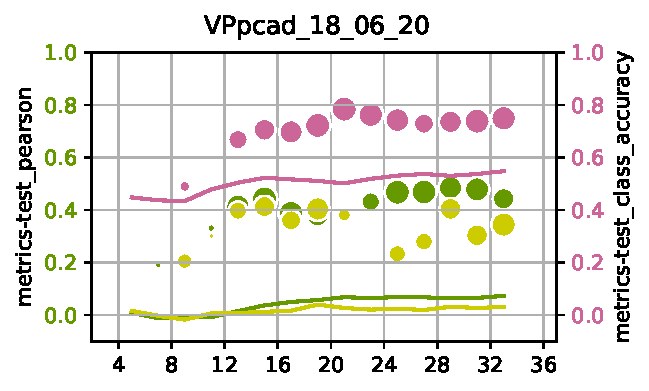
\includegraphics[width=\subplotwidth]{./figures/csp_spoc_incommon/bubble_csp_spoc_incommon_VPpcad_d2_nolegend}& & 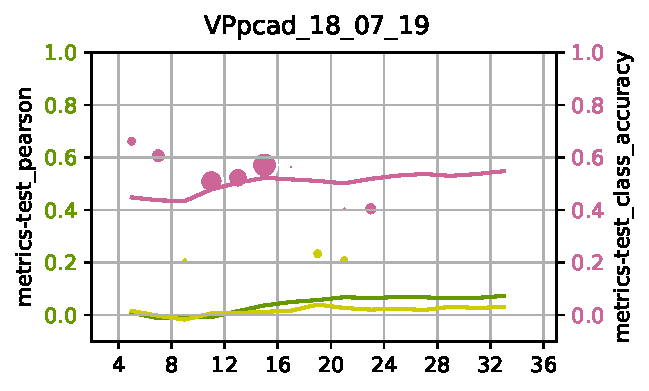
\includegraphics[width=\subplotwidth]{./figures/csp_spoc_incommon/bubble_csp_spoc_incommon_VPpcad_d4_nolegend}\\
& & 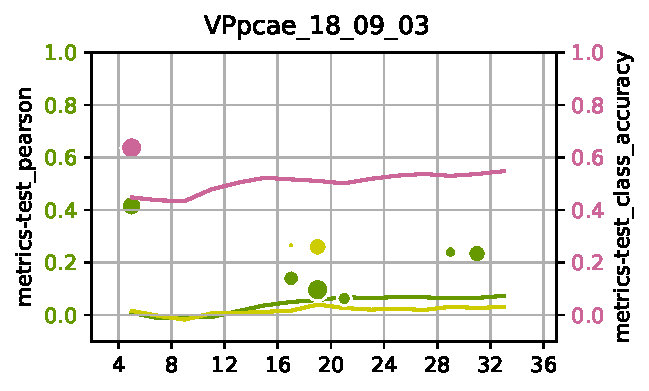
\includegraphics[width=\subplotwidth]{./figures/csp_spoc_incommon/bubble_csp_spoc_incommon_VPpcae_d4_nolegend}\\
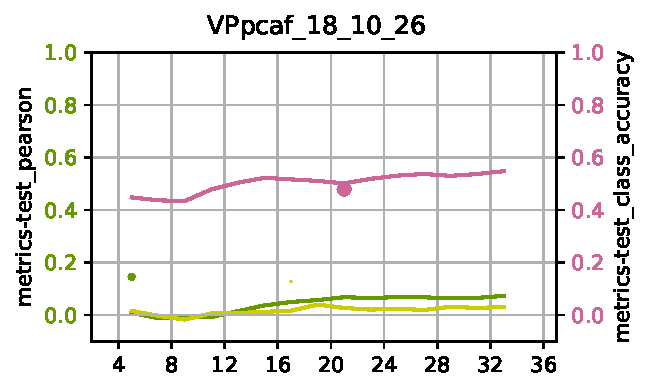
\includegraphics[width=\subplotwidth]{./figures/csp_spoc_incommon/bubble_csp_spoc_incommon_VPpcaf_d2_nolegend}& 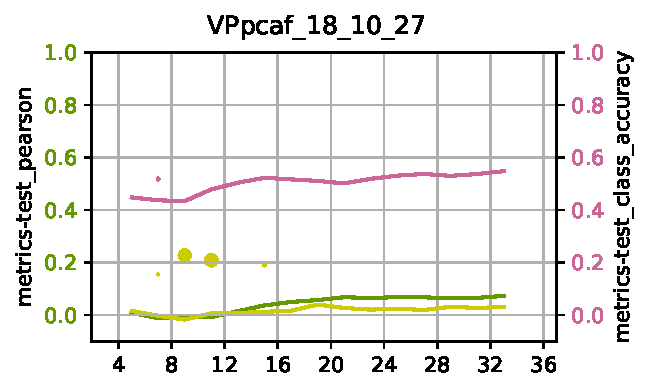
\includegraphics[width=\subplotwidth]{./figures/csp_spoc_incommon/bubble_csp_spoc_incommon_VPpcaf_d3_nolegend}& 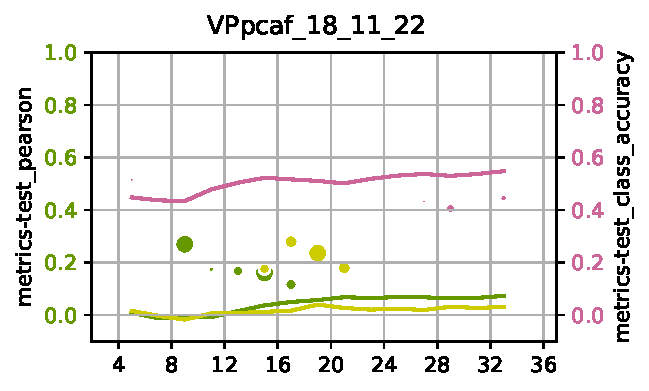
\includegraphics[width=\subplotwidth]{./figures/csp_spoc_incommon/bubble_csp_spoc_incommon_VPpcaf_d4_nolegend}\\
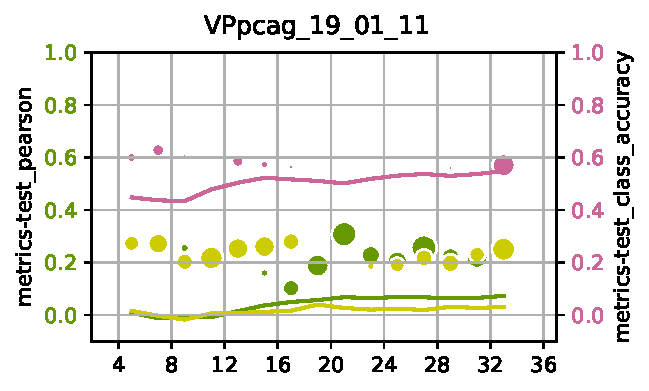
\includegraphics[width=\subplotwidth]{./figures/csp_spoc_incommon/bubble_csp_spoc_incommon_VPpcag_d2_nolegend}& 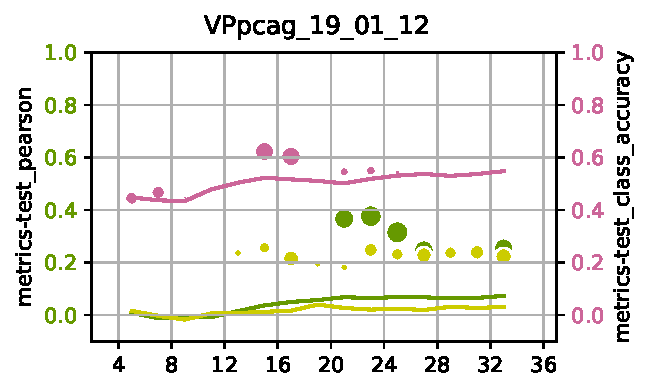
\includegraphics[width=\subplotwidth]{./figures/csp_spoc_incommon/bubble_csp_spoc_incommon_VPpcag_d3_nolegend}& 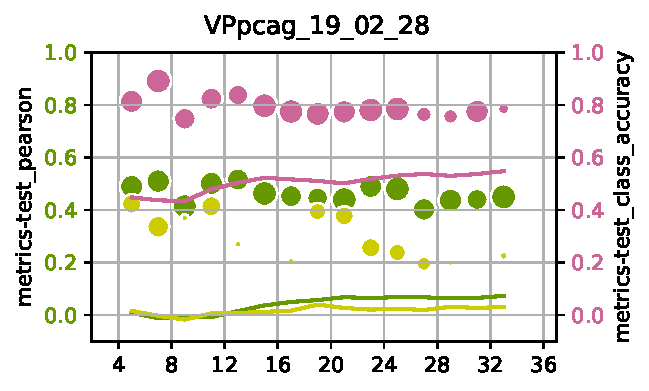
\includegraphics[width=\subplotwidth]{./figures/csp_spoc_incommon/bubble_csp_spoc_incommon_VPpcag_d4_nolegend}\\
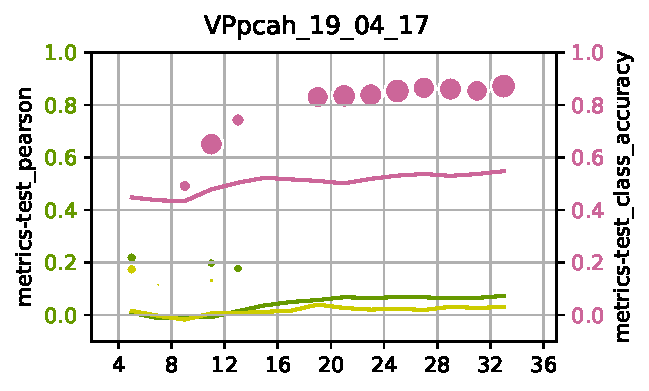
\includegraphics[width=\subplotwidth]{./figures/csp_spoc_incommon/bubble_csp_spoc_incommon_VPpcah_d2_nolegend}& & 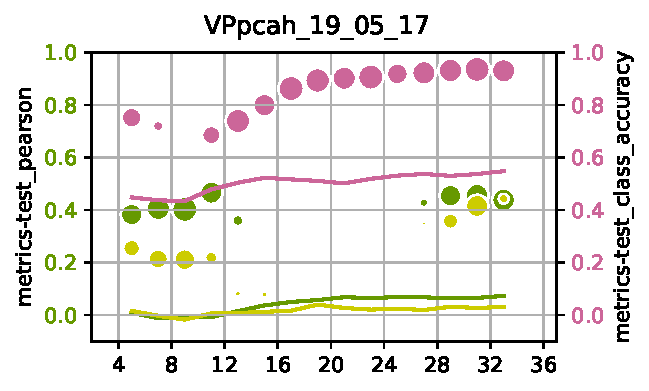
\includegraphics[width=\subplotwidth]{./figures/csp_spoc_incommon/bubble_csp_spoc_incommon_VPpcah_d4_nolegend}\\
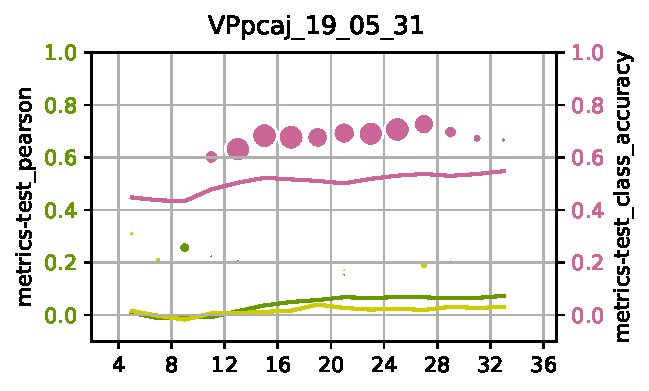
\includegraphics[width=\subplotwidth]{./figures/csp_spoc_incommon/bubble_csp_spoc_incommon_VPpcaj_d2_nolegend}& 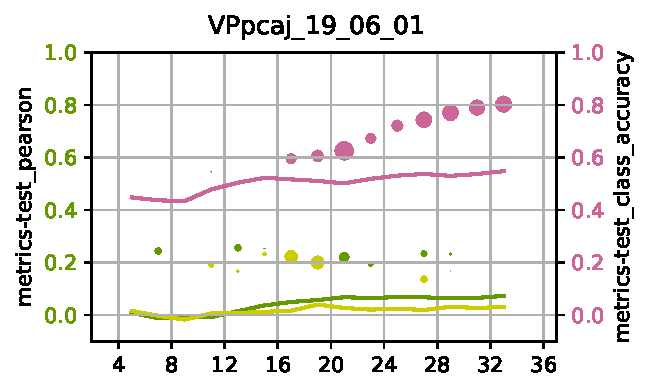
\includegraphics[width=\subplotwidth]{./figures/csp_spoc_incommon/bubble_csp_spoc_incommon_VPpcaj_d3_nolegend}& 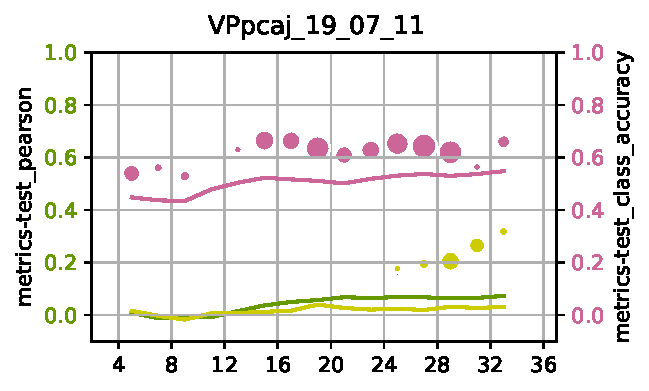
\includegraphics[width=\subplotwidth]{./figures/csp_spoc_incommon/bubble_csp_spoc_incommon_VPpcaj_d4_nolegend}\\
\end{tabular}
\caption{Motor performance}
\label{fig:decoding_performance_all}
\end{figure*}

Figure \ref{fig:decoding_performance_all} shows the decoding performance achieved for \regtask and  \classtask, evaluated in all sessions available. As baseline for the \regtask, we have included the decoding performance achieved by using the unsupervised method SSD. Additionally, the chance level for \regtask and  \classtask is shown as a solid line. The data-point size indicates the number of significant components found in the corresponding $f_c$. This can be interpreted as the  stability of a given frequency band as source of informative power-band features. The intuition behind this interpretation, is that a given component is able to deliver a consistently significant decoding performance, despite varying its $f_w$. An average of 45 different $f_w$ were computed for each of frequency bins shown.

For all sessions, relevant band-power features were found for \regtask and  \classtask, with the exception of \patient{4}{1}, \patient{4}{2}, where only few spurious components where discovered. Additionally for \regtask, sessions  \patient{2}{c} and \patient{7}{c} did not contain any relevant band-power features. Inversely, for \patient{4}{c} it was possible to find relevant features for \regtask in the alpha- and lower beta-bands, but none for \classtask.
 
For almost all sessions, frequency bands that are informative for \classtask, also derived in a good decoding accuracy for \regtask. Nevertheless a few exceptions are observed: For \patient{3}{c}, only theta-band features provided information for \classtask, whereas beta-band oscillations delivered significant decoding for \regtask. For \patient{5}{1}, informative features were found only in theta- lower beta-band for \classtask, whereas \regtask also profited from higher beta-band features. Higher frequency bands also delivered significant decoding performance for \regtask, but corresponded to components of muscular origin.

In \patient{6}{1}, besides relevant alpha-band components for both \regtask and \classtask, higher frequency bands contributed to a great decoding accuracy for \classtask, but not for \regtask. However, such components informative for \classtask correspond to DBS-artifacts. Similarly, for \patient{6}{c}, theta- and alpha band components provided relevant formation for decoding in \regtask and  \classtask, besides the DBS-elicited artifacts in higher frequency bands.

In \patient{7}{1}, alpha-band provided relevant formation for \regtask and \classtask, whereas higher beta-band was informative only for \classtask. Higher frequencies also provided discriminatory information for \classtask, however, they could be identified as of muscle-origin. For \patient{7}{2}, weakly predictive components for \regtask could be found in lower and higher beta-bands. For \classtask, relevant components could be found only in higher beta-band, followed by components of artifactual origin in higher frequency bands. For \patient{7}{c}, theta and lower beta components provided relevant information for \classtask. Higher frequency components also achieved good decoding performance for \classtask, but were of artifactual origin.

\begin{figure}
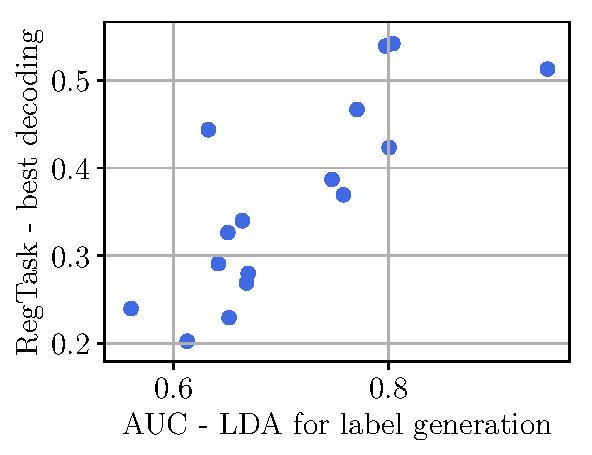
\includegraphics[width=0.24\textwidth]{figures/auclda_vs_bestdec}
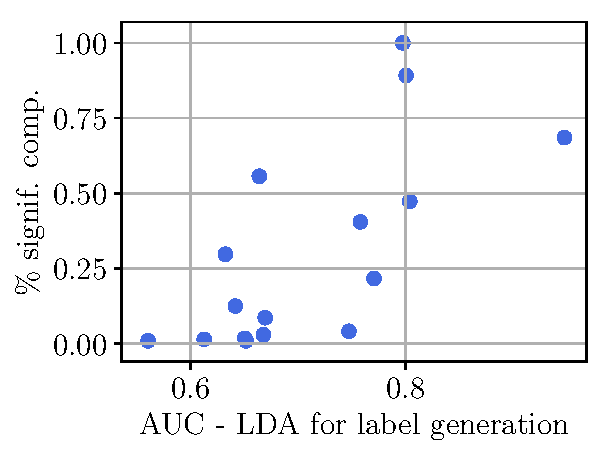
\includegraphics[width=0.24\textwidth]{figures/auclda_vs_ncomp}
\caption{Relation between AUC achieved when generating the LDA-based motor performance labels and: 1) the best decoding achieved in \regtask and 2) the percentage of significant components found for difference frequency bands. A significant linear correlation can be found in both cases.}
\label{fig:auclda_perf}
\end{figure}

Panel A of Figure \ref{fig:auclda_perf} shows the relationship between th behavioral contrast induced by DBS---quantified by the AUC obtain for the LDA-based label generation procedure--- and the maximum decoding performance between for \regtask. Similarly, Panel B shows the relation between the same DBS-induced behavioral contrast, and the percentage of significant components found during the random search performed for \regtask. There is a clear relation in both cases, which suggest that the DBS-induced behavioral contrast has a direct effect in decoding performance achievable for \regtask. We suggest to causes for this: first, according to \cite{AndreasComponentsStroked}, the variance of the labels has direct correlation with decoding performance achieved by SPoC. Second, if not major behavioral differences among trials can be elicited for what we hypothesize to be the major variance-inducing variable, i.e., DBS; then it can be assumed that the variance observe correspond to weak noise processes, not extractable from the EEG signals recorded.

\subsection{Spatial patterns common to \regtask and \classtask}

\subsection{Spatio-temporal signatures}
In the following, the spatio-temporal signatures of the significant components identified for the chronic sessions will be presented. We have excluded the acute sessions from this analysis since the incompleteness of the EEG layout precludes the interpretation of the spatial patterns obtained. Here, we refer to spatio-temporal signatures as the set of spatial patterns identified by SPoC, as well as the corresponding averaged ERD/ERS.

From all the components obtained, we have manually discarded components that can be attribute to artifacts. The criteria used for distinguishing artifact vs non-artifact was based on the same criteria used in ICA, i.e., take into account the spatio-temporal-spectral signatures of the components \cite{MARAOrSimilarHowToIdentifyArtifacts}. For clarity, Figure \ref{fig:artifacts}, show an subset of components selected as artifactual.

Two type of components are found for \patient{1}{c}: 1) a lateralized parietal component extracted from the alpha band, and 2) a central component extracted from low and high beta band. The former might be attributed to attention process, whereas the latter suggest an underlying motor process. Also interesting the parietal pattern, contains a \cpdt-trial time-locked ERS which is also modulated by stimulation, with an enhanced ERS under DBS-on. 

For \patient{2}{c}, a much smaller amount of significant components was found. In this case, the spatial patterns are not clearly of neural origin, however, their spectral signature shows a narrow-band enhancement of the beta-band power.

For \patient{3}{c} 

\patient{4}{c}, show a significant temporal-parietal component found the alpha band. This component also shows a \cpdt-trial time-locked ERD. This component does not show a difference between conditions DBS-on and -off.

The spatio-temporal signatures found for \patient{5}{c} are noteworthy: Here, an average correlation of $\approx0.5$ was achieved for left-hemisphere pre-frontal components extracted from the theta-band, which are enhanced for DBS-on. This suggests that for this patient, the stimulated part of the STN might have abundant projections to the prefrontal cortex.

As this cortical area is known to modulate cognitive processes, this result might be interpreted as a modulation of motor performance by an underlying cognitive process, instead of a motor process. Simmilar cases have been reported before, where DBS-induced impulsivity would lead to an increased speed in these type of tasks \cite{IMPULSIVITY DBS}

In \patient{6}{c}, we found an stereotypical alpha-band oscipital component. This might indicate an underlying attention process. 

Finally, similar to the patterns found for \patient{5}{c}, for \patient{7}{c} we found a frontal (non-lateralized) theta-band component which, contrary to \patient{5}{c}, was suppressed by DBS-on



%\todo{The patterns that dont show a difference between on/off in the spectrum... is it the same in the coarse spectrum?}
% R: There is a difference, although very very small. The difference is the same as observed in the fine spectrum.

\section{Discussion}






\section{Conclusions}


\bibliographystyle{apalike}
\bibliography{specific}


\end{document}